\chapter{Evaluation}

    There are two general criteria that metamorphic engines are generally
    evaluated on. The first is that the programs produced by the engine
    perform the same high level function as the original seed program. The
    second, is that all of the programs produced by the metamorphic engine
    exhibit a high degree of dissimilarity among each other at the byte
    level. The underlying goal here is the evasion of classical
    byte-signature based malware detection algorithms.

    In addition to evading traditional detection techniques, the second goal
    of this engine is to evade newer detection algorithms which rely on
    comparing the opcode histograms of ``normal'' programs with the
    histogram of the program being classified \cite{histogram}.

\section{Functional Equivalence}

    For a metamorphic engine to be useful it must claim to preserve the
    semantics of the seed program. In this implementation, each method of
    the seed program is encoded as a sequence of abstracted assembly-like
    statements. Each of these statements has a clear and well defined
    mapping to sequences of gadgets.
    
    During code generation, each method's statements are compiled down to a
    sequence of gadgets. In the process, local variables are mapped to
    memory locations and registers. The resulting byte-string for the method
    is generated by translating each gadget into bytes. This is done
    choosing an appropriated instance of the gadget in the library.

    To show that the code generation maintains the original semantics of the
    seed program, it is sufficient to show the following:

    \begin{enumerate}

        \item All of the byte-strings that a given gadget maps to have the
            same effect on the execution state.

        \item The sequences of gadgets corresponding to each statement
            preserve the semantics of that statement.

        \item Choice of registers and memory locations do not have an
            outwardly observable effect on execution state.

    \end{enumerate}

    \subsection{Functional Equivalence of Byte-strings}
    \label{sec:results-gadget-inst-eq}

        %TODO: This section still needs some work

        The guarantee of functional equivalence of byte-strings for a
        particular gadget in the library is a direct result of the
        conservative design of both the abstract evaluator and the gadget
        discovery algorithm.

        The abstract evaluator only successfully evaluates \emph{x86} instructions
        that have a deterministic effect on the execution state.  Meaning
        that the resulting state of every hardware location
        \footnote{Hardware locations are defined as registers, flags and
        memory addresses.} can be described algebraically \footnote{Without
        the use of conditional operators.} in terms of the original values
        of the hardware locations prior to execution. Examples of states
        that cannot be represented in this model include the effect of
        instructions following a conditional branch, and any sequence of
        instructions that perform multiple indirect writes to memory.

        Confining the space of allowed execution states in this manner
        allows the resulting execution state to be represented as a
        collection of algebraic expression trees, with exactly one tree for
        each modified location. Matching bytes to gadgets is done by
        attempting to match one the resulting expression trees to the target
        trees defined for each class of gadget. The hardware locations whose
        corresponding trees are not included in the match are recorded in
        the clobber set, which fully accounts for the side-effects of the
        match.

        There are several restrictions placed on the expression that are
        allowed to be placed in the clobber set. This is done to simplify
        the verification that a given byte-string does not have unaccounted
        for effects on hardware. States that include indirect memory
        accesses (unless explicitly required by the gadget, e.g.
        \emph{LoadMemReg} and \emph{StoreMemReg}) are are disqualified from
        being included in the library as writes and reads from unmapped
        address result in undefined behaviour.
        
        The only allowed side effects of a gadget is the clobbering of
        general purpose registers with either constant values or values from
        other registers. This ensures that gadgets only perform safe
        operations and that they can be fully described by the gadget's
        pre/post-conditions and the list of clobbered register locations.

        %The abstract evaluator only evaluates a very small subset of the
        %full x86 instruction set. The evaluation of any instruction not so
        %defined results in an invalid execution state. Further each
        %instruction handled by the abstract evaluator only results in a
        %valid execution state if all of the side effects of the instruction
        %can be easily expressed in terms of the initial execution state.
        %For instance instructions following conditional jumps, and
        %instruction sequences that perform multiple indirect writes to
        %memory result in invalid execution states because they have
        %nondeterministic side-effects.

    \subsection{Gadget/Statement Equivalence \& Irrelevance of Specific Registers}

        Every local variable defined by a method is mapped to memory
        locations at positive and negative offsets from the EBP register
        corresponding to method input and local variables respectively. The
        mapping of local variables to memory locations is static and does
        not change over the course of the program.

        Each statement has a core semantic that maps to specific gadgets. In
        the case of this implementation each statement corresponds to a
        single core gadget operation\footnote{For instance the \emph{add}
        statement's core semantic corresponds to the \emph{Plus} gadget.}.
        Given this it is possible to define the operational semantics of a
        statement as the gadget that implements it.

        To fully execute a statement the values or constants that constitute
        the statement's parameters must be loaded into temporary registers so
        that they may be used with the corresponding gadget\footnote{Unless
        required by the semantics of the gadget, each gadget only operates
        on register locations. The only gadgets in this implementation that
        operate on values other than registers are \emph{LoadMemReg},
        \emph{StoreMemReg}, and \emph{LoadConst}}.  This is done through the
        \emph{LoadMemReg} and \emph{LoadConst} gadgets.  After the necessary
        values have been loaded into temporary registers, another temporary
        register is allocated for the result of the operation if applicable
        and the core gadget is performed on the temporary registers.  If the
        result is intended to be saved the temporary register corresponding
        to the results is placed back into the abstract location through a
        \emph{StoreMemReg} gadget.
        
        Temporary registers are allocated for the duration of the
        statement's execution and are temporarily removed from the pool of
        unallocated general registers. When translating gadgets into
        concrete bytes, only those instances whose clobber list is a subset
        of the current unallocated register pool are considered valid
        translations. Because the side-effects of gadgets are limited to
        altering values in unallocated general purpose registers, the
        observable\footnote{An observable effect being one that alters the
        value of an allocated temporary register, the value of a memory
        location, or altering the instruction pointer} effect on the
        execution state can be described by the pre/post-conditions of the
        sequence of gadgets, which is by definition the semantics of the
        statement.
    
\section{Test Suite}

    The next two sections describe experiments intended to measure the
    performance of the metamorphic engine against detection techniques
    resembling real world algorithms.

    A gadget library was pregenerated using each of the described byte
    sources.  The method presented in \cite{franken} is referred to as
    ``Frankenstein'', the naive approach of sampling bytes from a uniform
    distribution is referred to as ``Uniform Random'', and the proposed
    method of sampling bytes from the observed byte frequency distribution
    of windows programs is referred to as ``Observed Random''.

    Three simple test programs are provided as seeds for the engine.
    Descriptions of the sample programs are given below, and the source code
    for each is given in appendix~\ref{app:test-program-source}. A
    collection of 100 programs was then generated for each combination of
    test program and gadget library.
    
    \subsection{Sample Programs}

        \subsubsection{Max}

            The max program is a very simple method that takes as input two
            signed integers and returns the greater of the two. The purpose
            of the max program is to test value returning and forward
            conditional jumps (if statements).

        \subsubsection{Factorial}

            The factorial program takes as input a signed integer and
            returns a signed integer corresponding to the factorial of the
            input. The calculation is done inside a loop. The factorial
            program is intended to test various arithmetic gadgets along
            with backward conditional jumps.

        \subsubsection{Xor}

            The xor program defines a method that receives as input a
            pointer to an array of signed integers, the length of the array,
            and an integer valued key. The method iterates through the array
            xoring each value with the supplied key. Along with performing a
            task commonly seen in polymorphic malware, this method also
            demonstrates the ability to dereference memory locations, and
            the ability to control flow through conditional jumps.
        
\section{Metamorphic Variety}
    
    The following experiment is intended to evaluate the performance of the
    engine in a scenario closely resembling traditional byte-signature based
    detection techniques. In order to evade these techniques, the generated
    programs must exhibit a degree of variation in their opcodes.

    Accordingly, the evaluation metric for this experiment is modelled after
    the system presented in \cite{cfg_lcs} which uses the longest common
    subsequence (LCS) as its basis. The metric described in \cite{cfg_lcs}
    is concerned with the sequences of opcodes in the basic blocks of the
    control flow graph and yields a value from $0$ to $1$ corresponding to
    the percent of overlap in corresponding basic blocks in the control flow
    graph.
    
    Given that our metamorphic engine does not support basic block
    reordering as one of it's obfuscation techniques it follows that
    corresponding basic blocks in each variant will appear in the same
    relative ordering in the generated code. Therefore the metric has been
    adapted to take advantage of this simplification.

    \begin{figure}[t]
        \makebox[\textwidth][c]{ 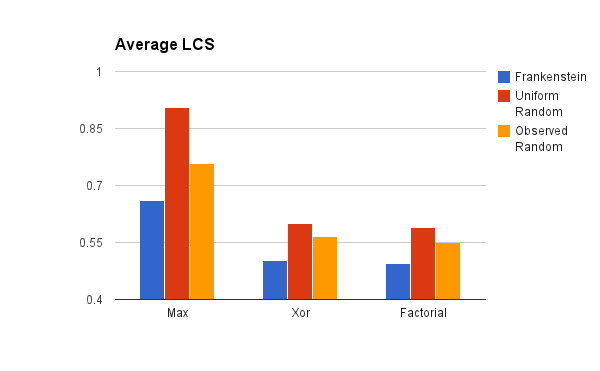
\includegraphics[width=1.10\textwidth]{chart_lcs.png} }
        \vspace{-50pt}
        \caption{Similarity scores for the each combination of test program
        and gadget library. Lower scores are more desirable, a score of $1$
        indicates that the programs are identical, while $0$ indicates that
        there is no overlap.}
        \label{tab:results-different}
    \end{figure}
%%        \begin{table}
%%            \centering
%%            \begin{tabular}{|c||c|c|c|}
%%                \hline
%%                                & Xor & Factorial & Max \\
%%                \hline
%%                Uniform Random  & 0.6004 & 0.5901 & 0.9061 \\
%%                \hline
%%                Sampled Random  & 0.5654 & 0.5507 & 0.6593 \\
%%                \hline
%%                File Scanning   & 0.5026 & 0.4941 & 0.7582 \\
%%                \hline
%%            \end{tabular}
%%            \caption{Similarity scores for the each combination of test program
%%            and gadget library. Lower scores are more desirable, a score of $1$
%%            indicates that the programs are identical, while $0$ indicates that
%%            there is no overlap.}
%%            \label{tab:results-different}
%%        \end{table}
%%
    The similarity score between two methods is defined to be the percent of
    the total opcodes among the two methods that are present in their longest
    common subsequence. The formula is defined as follows, where
    $A$ and $B$ are the lists of opcodes making up the two methods,
    $LCS(A,B)$ is the length of their longest common subsequence, and $|A|$,
    and $|B|$ are the length of $A$ and $B$:

    $$Sim(A,B) = \frac{LCS(A,B)}{|A| + |B| - LCS(A,B)}$$

    The score for each combination of gadget library and test program is
    calculated by averaging each pairwise similarity score among the 100
    generated samples.  The resulting scores are shown in
    figure~\ref{tab:results-different}. 

\section{Appearing Normal}

    The following experiment is intended to measure the effectiveness of
    this engine against detection techniques that rely on comparing the
    opcode histograms of suspected malware against opcode histograms of
    ``normal'' Windows programs.

    Due to the potential ambiguity of what constitutes a normal Windows
    program, we chose a very conservative definition and built the opcode
    frequency distribution from executables contained in a vanilla install
    of the Windows operating system. In particular, the distribution was
    generated from each {.dll} and {.exe} in the subdirectories of the
    \emph{C:/Program Files/} folder found in a fresh install of the 32-bit
    version of Microsoft Windows 7 Ultimate. The resulting distribution is
    built from a total of $248$ files and the most frequent $32$ opcodes are
    given in table~\ref{tab:results-windows-dist}.

    \begin{table}
        \centering
        \begin{tabular}{|c|c||c|c||c|c||c|c|}
            \hline
            Opcode & Freq & Opcode & Freq & Opcode & Freq & Opcode & Freq \\
            \hline
            add & 0.2184 & or & 0.0256 & outsd & 0.0137 & popad & 0.0090 \\
            \hline
            mov & 0.1188 & inc & 0.0205 & dec & 0.0137 & jae & 0.0089 \\
            \hline
           push & 0.1060 & lea & 0.0204 & jb & 0.0136 & ret & 0.0082 \\
            \hline
           int3 & 0.0447 & sub & 0.0202 & jmp & 0.0129 & sbb & 0.0073 \\
            \hline
           call & 0.0343 & and & 0.0176 & jnz & 0.0121 & insb & 0.0068 \\
            \hline
            pop & 0.0309 & xor & 0.0168 & imul & 0.0110 & invalid & 0.0062 \\ 
            \hline
             jz & 0.0286 & adc & 0.0159 & outsb & 0.0097 & arpl & 0.0055 \\ 
            \hline
            cmp & 0.0260 & test & 0.0145 & nop & 0.0093 & jo & 0.0052 \\
            \hline
        \end{tabular}
        \caption{The distribution of opcodes in normal Windows programs.}
        \label{tab:results-windows-dist}
    \end{table}

    The notation of classifying families of programs and files through
    frequency distributions has a strong president in literature
    \cite{chisquared,hmm_evade,stat_model,fileprints}. The basis for our
    evaluation is the classification system described in \cite{chisquared}
    which uses Pearson's chi-squared test for goodness of fit to measure the
    likelihood that a file under consideration belongs to a particular
    family of programs.

    Pearson's chi-squared test for goodness of fit tests the hypothesis that
    an observed frequency distribution matches a given theoretical
    distribution. The theoretical distribution in the case of malware
    classification is the frequency distribution of opcodes in a specific
    family of executables. In \cite{chisquared} families of executables
    refers to various strains of metamorphic malware, in our case the family
    of programs we care about is the family of normal Windows executables.
    
    %For use with the chi-squared tests, families of programs are defined as
    %a probability distribution with parameter $\theta \in \mathbb{N}^{255}$,
    %where $\theta_i$ corresponds to the counts of given byte value $i$
    %occurring in a program.

    The chi-squared test statistic, $X^2$, is defined by the following
    equation, where $O_i$ is the observed frequency of opcode $i$ in the
    sample, $E_i$ is the expected frequency, and $n$ is the total number of
    unique categories.

    $$X^2 = \sum_{i=0}^{n} \frac{(O_i - E_i)^2}{E_i}$$

    After the test statistic $X^2$ is calculated it is compared to the
    p-value of the chi-squared distribution parameterized with the
    appropriate degrees of freedom and false-positive error rate. If the
    calculated $X^2$ is less than the p-value then the hypothesis is
    accepted.

    In general the degrees of freedom is equivalent to one minus the number
    of categories, in this case it is $559$ which corresponds to one less
    than the number of unique opcodes in the \emph{x86} instruction space
    recognized by our disassembler. The false positive rate generally
    accepted as statistically significant and suggested by \cite{chisquared}
    is $0.05$.

    \begin{figure}[t!]
        \makebox[\textwidth][c]{ 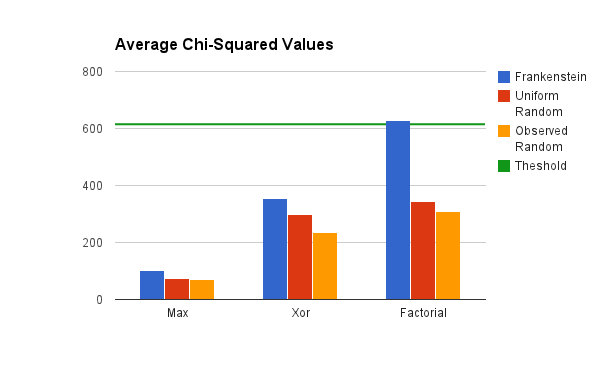
\includegraphics[width=1.10\textwidth]{chart_x2.png} }
        \vspace{-50pt}
        \caption{The average $X^2$ values of all generated instances for
            each combination of sample program and library. Lower numbers
            indicate a stronger similarity with the observed windows opcode
            distribution}
        \label{tab:results-windows-like-avg}
    \end{figure}

    \begin{table}
        \centering
        \begin{tabular}{|c||c|c|c|c|c|c|}
            \hline
                            & Xor & Factorial & Max \\
            \hline
            Uniform Random  & 100\% & 100\% & 100\%\\
            \hline
            Sampled Random  & 100\% & 100\% & 100\%\\
            \hline
            File Scanning   & 97\% & 52\% & 100\% \\
            \hline
        \end{tabular}
        \caption{The percent of generated examples from each combination
            that were classified as benign.}
        \label{tab:results-windows-like-passed}
    \end{table}

    The corresponding p-value with this parameterization is $615.11$. This
    means that any $X^2$ values less than $615.11$ indicates that the sample
    program belongs to the family of normal Windows programs.
    Figure~\ref{tab:results-windows-like-avg} presents the average $X^2$
    values for each combination of library and sample program.
    Table~\ref{tab:results-windows-like-passed} gives the percent of
    generated examples that are classified as benign by comparison to the
    p-value.

    %http://www.danielsoper.com/statcalc3/calc.aspx?id=12
    %293.24

    %df = 559
    %my $_CHI2_MAX = 615.11150122;
